% !TEX TS-program = lualatex+se+debug
% !TEX encoding = UTF-8 Unicode

\documentclass[14pt, twoside, a4paper]{extreport}
% -----------------------------------------------------------------------------------
% ------------------------- USTAWIENIA STRONY--------------------------
% -----------------------------------------------------------------------------------
\usepackage{geometry}
\geometry{
	left=10mm,
	right=10mm,
	top=15mm,
	bottom=15mm,
	marginparwidth=0mm,
	marginparsep=0mm
	}
\newcommand{\wstawplik}[1]{\input{../include/#1}}%skraca kod
\wstawplik{headerofficium}
% elementy zmienne co do headerofficium:
\graphicspath{{../img/}} % katalog obrazów
\grechangestaffsize{20}%rozmiar wyniku GregorioTEX
% koniec 

% debugowanie:
% %\iffalse %*** %\fi %***
% \tracingall przed problematycznym kodem - bardzo dużo informacji
% lualatex+se+debug - dodatkowe opcje: -file-line-error i -halt-on-error 
% \errorcontextlines

\begin{document}
% -----------------------------------------------------------------------------------
% ------------------------- STRONA TYTUŁOWA  --------------------------
\thispagestyle{empty}
\begin{center}
	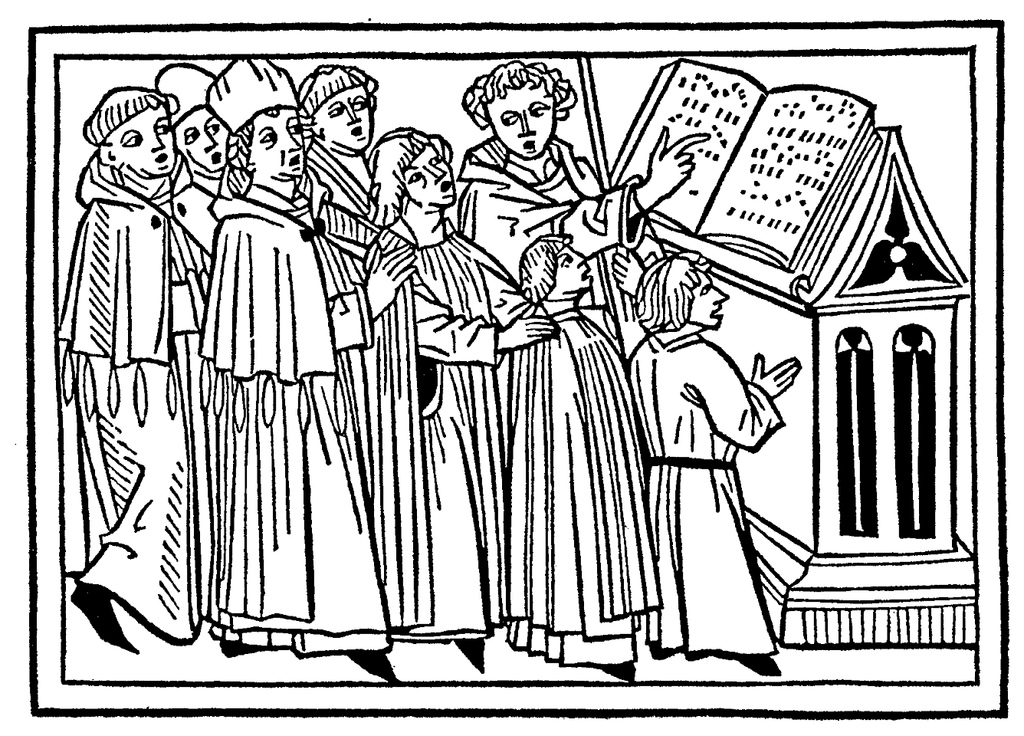
\includegraphics[width=1.0\linewidth]{singers_okładka.jpg}
	\vfill
	\tytulfont{COMPLETORIUM}
	\vfill
	\podtytulfont{Kompleta niedzielna\\wraz\\z~modlitwami wieczornymi}
	\vfill
	\large\textit{Liber usualis, Solesmes, 1961, p.262}
\end{center}%
\newpage
%\thispagestyle{empty}
\wstawplik{aperi_domine}
\setcounter{page}{1}
\fancyhead{}% wyczyść wszystkie pola nagłówka
\pagestyle{plain}% nagłówek i stopka pusta - UWAGA: przedefiniowany styl przez polecenie fancypagestyle w header.tex	
%\setlength{\parindent}{0pt}
\gresetbracerendering{font}
\sectionspace
\separator
\sekcja{Incipit}{Wszyscy wstają. Lektor wychodzi na środek, przyklęka i skłaniając się w kierunku ołtarza prosi o błogosławieństwo. W~obecności kapłana: ``Jube domne benedicere''~w jego kierunku. Błogosławieństwo - odpowiada kapłan lub pod jego nieobecność hebdomadariusz.}
\gresetinitiallines{0}\gabcsnippet{(c3)<c><sp>V/</sp>.</c> Ju([alt:Lector]h)be(h) Do(h)mi(h)ne(g'_) be(h)ne(h)di(h)ce(d)re(f.::)}
\vspace{-5mm}
\tlumaczR{\Vbar. Pobłogosław, ojcze.}\segmentspace% 
\gresetinitiallines{0}\gabcsnippet{(c3)Noc([alt:Benedictio]h)tem(h) qui(h)ét(h)am(h) et(h) fi(h)nem(g) per(f)féc(h)tum(h.;) con(h)cé(h)dat(h) no(h)bis(h) Do(h)mi(h)nus(h) o(h)mni(h)po(d)tens(d.::) <c><sp>R/</sp>.</c> A([alt:Chorus]g.)men(h.::)}
\tlumaczR{Noc spokojną i koniec doskonały niech nam da Pan wszechmogący. \Rbar. Amen.}\segmentspace% 
\gresetinitiallines{1}\grecommentary{1 Petr. 5, 8-9}\gabcsnippet{(c3) Frá([alt:Lector]h)tres:(h.)(,) Só(h)bri(h)i(h) e(h)stó(h)te(h), et(h) vi(h)gi(h)lá(h)te:(f.;) qui(h)a(h) a(h)dver(h)sá(h)ri(h)us(h) vés(h)ter(h) diá(h)bo(h)lus,(h'_)(,) tam(h)quam(h) lé(h)o(h) rú(h)gi(h)ens,(h'_)(,) cír(h)cu(h)it(h), quaé(h)rens(g) quem(f) dé(h)vo(h)ret:(h.;) cú(h)i(h) re(h)sí(h)sti(h)te(h) fór(h)tes(h) in(h) fí(h.)de.(d.:) Tu(h) au(g)tem(f) Dó(h)mi(h)ne(h._), mi(h)se(h)ré(h)re(h) nó(h.)bis.(d.::) <c><sp>R/</sp>.</c> De([alt:Chorus]h)o(h) grá(h)ti(d)as.(d.::)}
\tlumaczR{Bracia: Trzeźwymi bądźcie, a czujcie: boć przeciwnik wasz djabeł jako lew ryczący krąży, szukając, kogoby pożarł: któremu się sprzeciwiajcie mocni w wierze. \Vbar. Ty zaś, Panie, zmiłuj się nad nami. \Rbar. Bogu niech będą dzięki.}\segmentspace% 
\gresetinitiallines{0}\gabcsnippet{(c3) <c><sp>V/</sp>.</c> Ad(h[alt:Hebdomadarius])ju(h)to(h)ri(h)um(h) nos(h)trum(h) <c><v>\grecross</v></c> in(h) no(h)mi(h)ne(h) Do(h)mi(f)ni(f) (::) <c><sp>R/</sp>.</c> Qui fe(h[alt:Chorus])cit(h) cae(h)lum(h) et(h) ter(h)ram.(f') (::)}
\tlumaczR{\Vbar. Wspomożenie nasze \grecross w imieniu Pana. \Rbar. Który stworzył niebo i ziemię.}
\newpage
\rubryka{Odmawia się \emph{Pater noster} po cichu, oraz czyni rachunek sumienia. W przypadku obecności kapłana, może on poprowadzić rachunek sumienia, wówczas pierwszy odmawia  \emph{Confiteor}, a~następnie wszyscy (analogicznie jak przy modlitwach u stopni ołtarza).}
\BeginParallel
\latN{\inicjal{P}{ater} noster, qui es in cælis, sanctificétur nomen tuum: advéniat regnum tuum: fiat volúntas tua, sicut in cælo et in terra. Panem nostrum quotidiánum da nobis hódie: et dimítte nobis débita nostra, sicut et nos dimíttimus debitóribus nostris: et ne nos indúcas in tentatiónem: sed líbera nos a malo. Amen.}\pol{\inicjal{O}{jcze} nasz, któryś jest w niebie, święć się imię Twoje: przyjdź królestwo Twoje: bądź wola Twoja, jako w niebie tak i na ziemi. Chleba naszego powszedniego daj nam dzisiaj: i odpuść nam nasze winy, jako i my odpuszczamy naszym winowajcom: i nie wódź nas na pokuszenie: ale nas zbaw ode złego. Amen.}%

\latN{\inicjal{C}{onfíteor} Deo omnipoténti, beátæ Maríæ semper Vírgini, beáto Michaéli Archángelo, beáto Joánni Baptístæ, sanctis Apóstolis Petro et Paulo, et ómnibus Sanctis, quia peccávi nimis, cogitatióne, verbo et ópere: mea culpa, mea culpa, mea máxima culpa. Ídeo precor beátam Maríam semper Vírginem, beátum Michaélem Archángelum, beátum Joánnem Baptístam, sanctos Apóstolos Petrum et Paulum, et omnes Sanctos, oráre pro me ad Dóminum Deum nostrum.}\pol{\inicjal{S}{powiadam} się Bogu wszechmogącemu, Najświętszej Maryi zawsze Dziewicy, świętemu Michałowi Archaniołowi, świętemu Janowi Chrzcicielowi, świętym Apostołom Piotrowi i Pawłowi, i wszystkim Świętym, że bardzo zgrzeszyłem, myślą, mową i uczynkiem: bijąc się w piersi moja wina, moja wina, moja bardzo wielka wina. Przeto błagam Najświętszą Maryję zawsze Dziewicę, świętego Michała Archanioła, świętego Jana Chrzciciela, świętych Apostołów Piotra i Pawła, i wszystkich świętych, o modlitwę za mnie do Pana Boga naszego.}%

\latN{\inicjal{M}{isereátur} nostri omnípotens Deus, et dimíssis peccátis nostris, perdúcat nos ad vitam ætérnam. Amen.}\pol{\inicjal{N}{iech} się zmiłuje nad nami Bóg wszechmogący, a odpuściwszy nam grzechy, doprowadzi nas do życia wiecznego. Amen.}%

\latN{\inicjal{I}{ndulgéntiam}, \grecross~absolutiónem et remissiónem peccatórum nostrórum tríbuat nobis omnípotens et miséricors Dóminus. Amen.}\pol{\inicjal{P}{rzebaczenia}, \grecross~rozgrzeszenia i odpuszczenia grzechów naszych, niech nam udzieli Pan wszechmogący i miłosierny. Amen.}%
\EndParallel
\rubryka{Czyni się znak krzyża na klatce piersiowej.}
\gresetinitiallines{0}\gabcsnippet{(c3) <c><sp>V/</sp>.</c> Con(h[alt:Hebdomadarius])vér(h)te(h) nos(h) <c><v>\grecross</v></c> Déus(h) sa(h)lu(h)tá(g)ris(f) nó(h)ster(h) (::) <c><sp>R/</sp>.</c> Et(h[alt:Chorus]) a(h)vér(h)te(h) í(h)ram(h)  tú(h)am(g) a(f) nó(h)bis.(h) (::)}
\tlumaczR{\Vbar. Nawróć nas \grecross~Boże, nasz zbawco.. \Rbar. I odwróć swój gniew od nas.}
\gresetinitiallines{0}\gabcsnippet{(c3) <c><sp>V/</sp>.</c> De(h)us(h'_) (,) in(h) ad(h)ju(h)tó(i)ri(h)um(h) me(h)um(h'_) in(h)tén(g)de.(h.) (::) <c><sp>R/</sp>.</c> Dó(h)mi(h)ne(h'_) (,) ad(h) ad(h)ju(h)ván(h)dum(h) me(h'_) fe(h)stí(g)na.(h.) (:) Gló(h)ri(h)a(h) Pa(h)tri,(h) et(h) Fí(h)li(h)o,(h'_) (,) et(h) Spi(h)rí(h)tu(h)i(h) San(g)cto.(h.) (:) Sic(h)ut(h) e(h)rat(h) in(h) prin(h)cí(h)pi(h)o,(h) et(h) nunc,(h) et(h) sem(h)per,(h.) (,) et(h) in(h) saé(h)cu(h)la(h) sae(h)cu(h)ló(h)rum.(h) A(g)men.(h.) (;) Al(h)le(i)lú(hg~){ia}.(g.) (::) (Z)
<i>Vel :</i>() Laus(h) ti(h)bi(h) Dó(h)mi(h)ne(h'_) Rex(h) ae(h)tér(h)nae(i) gló(h')ri(h)ae.(g.) (::)}

\sekcja{Modlitwy końcowe}{Odmawia się po cichu w pozycji klęczącej.}
\sloppy
\wstawplik{modlitwy_koncowe_credo}

\end{document}